\chapter{General Purpose Input/Outputs}

TODO: Pins and ports

One of the simplest ways to interface the microcontroller with external circuitry is via GPIO. Most pins on the microcontroller are able to operate in GPIO mode. As the name implies, a GPIO pin can be either an input or an output. Additionally, a pin can be placed into an alternate function or analogue mode; these will be discussed later.

A diagram showing how the pin is structured electrically inside the microcontroller is shown in \autoref{fig:gpio}. The ability for the microcontroller to communicate with external devices via GPIO pins is one of the defining differences between microcontrollers and microprocessors.

\begin{figure}
\centering
\includegraphics[page=152, clip=true, trim=90 410 90 210, width=\textwidth]{./stm32f0xx_reference_manual}
% left, bottom, right, top
\caption{Internal structure of pin. Source: Figure 17, Reference Manual}
\label{fig:gpio}
\end{figure}

%\begin{overpic}[grid,page=152, trim=90 410 100 210, clip, width=\textwidth]{./stm32f0xx_reference_manual}
%\end{overpic}

\section{Pin Mode}
As mentioned, the pin can be in one of four possible modes: input, output, alternate function, analogue. There is a register which controlled which mode the pin operates in, known as the GPIOx\_MODER. The 32 bits of the register are divided up into pairs of bits where each pair of pits sets the mode for the associated pin. 

\subsection{Input Mode}
Input mode is the default mode for most pins. In this mode, the pin is measuring the voltage applied to it and ascertaining whether it is a logic 0 or a logic 1. This 'decision' is made by a Schmitt Trigger which has useful things such as well defined high and low levels, hysteresis and high impedance. The logic level of each pin is latched on each clock cycle and written to the Input Data Register (GPIOx\_IDR). As each pin can only be considered to be either a logic high or a logic low, there is only 1 bit necessary to represent the state of a pin.

\subsection{Output Mode}
Here, the pin does not measure a logic level, but rather asserts a logic level. When in output mode, the pin will either assert a logic 0 allowing it to sink current from an external source, or assert a logic 1 allowing it to source current into an external sink. The logic level which is asserted is controlled by the Output Data Register (GPIOx\_ODR). 

\subsubsection{How to set or clear individual bits}
There is often a case where you wish to modify only one or two of the bits of a port, leaving the rest of the pins unchanged. If you simply write a pre-defined value to the pins, it will force \emph{all} of them to take on a specific value. The way to modify only a single bit is to do a logic AND or OR of the contents of the register with a pre-defined pattern. An OR has the ability to set specific bits while leaving others unchanged, while and AND has the ability to clear certain bits while leaving the others unchanged. For example, say we wanted to set bits 1 and 2, while clearing bits 0, 3, 4 and 5, leaving the other bits of the port unchanged. We could do something like the following:
\begin{lstlisting}[fontadjust=true,frame=trBL]
@ assuming Rn contains the address of the register to modify:
LDR R0, [Rn]    
LDR R1, =0b11111111111111111111111111000110
ANDS R0, R0, R1
MOVS R1, #0x06
ORRS R0, R0, R1
STR Rt, [Rn]
\end{lstlisting}


Each bit in this register can be set by writing to the register. Additionally, the bits in this register can be set via the Bit Set and Reset Register (GPIOx\_BSSR). This register allows atomic (done in a single instruction) setting or clearing of individual bits in the ODR. 
